\subsection{Motivation-to-Design Traceability}
This subsection focuses on design traceability, not on claiming cross-language performance gains. We define a four-stage traceability chain:
\begin{itemize}
\item \textbf{E0 (evidence assembly):} collect multilingual emergency-vs-normal acoustic evidence under a fixed mapping contract and dataset registry.
\item \textbf{E1 (shared-signal extraction):} identify stable shared features and quantify pooled effects with uncertainty and heterogeneity.
\item \textbf{E2 (design injection):} map shared acoustic signals to class-aware augmentation and an auxiliary stats branch.
\item \textbf{E3 (implementation check):} verify that training behavior remains consistent with the intended motivation-to-design path.
\end{itemize}
The purpose of E0--E3 is to make each design choice auditable back to source evidence files (\texttt{final\_report\_en\_2026w14.md}, \texttt{feature\_effects\_by\_language\_2026w14.csv}, \texttt{shared\_features\_meta\_2026w14.csv}, \texttt{divergence\_features\_2026w14.csv}, and \texttt{training\_preprocessing\_recommendations\_2026w14.md}).

\begin{figure}[t]
  \centering
  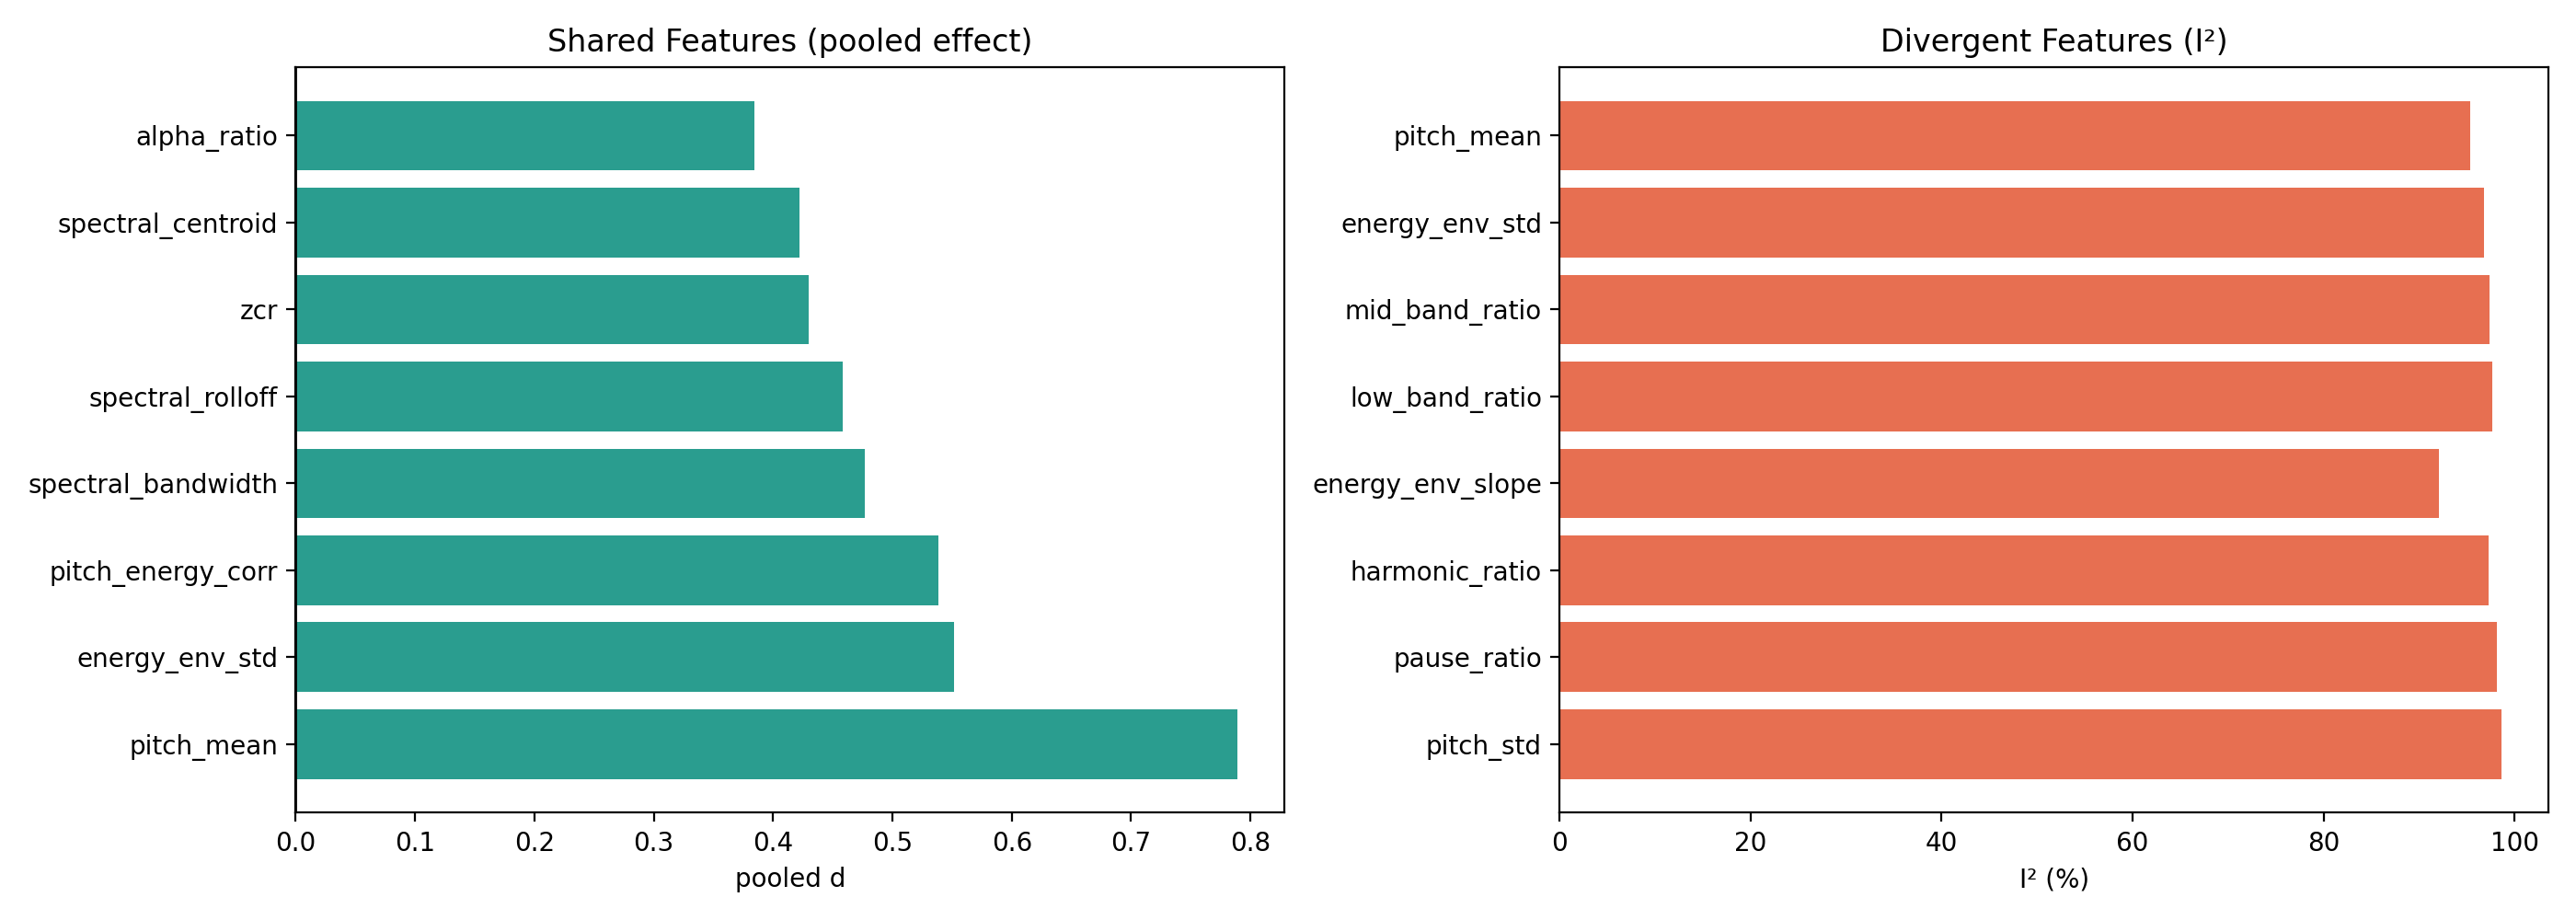
\includegraphics[width=\linewidth]{analysis/cross_language_emergency/longrun_multilingual_commonality_2026w14/figures/fig08_shared_vs_divergent_summary.png}
  \caption{Shared-vs-divergent summary used for motivation-to-design traceability (E0--E3).}
  \label{fig:traceability_shared_divergent}
\end{figure}

Additional diagnostics are included as supporting material and are intentionally de-emphasized in the main narrative: sample coverage (fig01), band-energy comparison (fig04), alpha-ratio comparison (fig05), centroid/bandwidth comparison (fig06), and pitch-energy-envelope comparison (fig07). These figures provide context for reproducibility and inspection, while Fig.~\ref{fig:traceability_shared_divergent} remains the main summary for design traceability.
For supplementary inspection (without changing the main claim scope), we refer readers to the additional files at the end of this section: \texttt{fig01\_sample\_coverage\_by\_language.png}, \texttt{fig04\_frequency\_band\_energy\_comparison.png}, \texttt{fig05\_alpha\_ratio\_multilingual.png}, \texttt{fig06\_centroid\_bandwidth\_multilingual.png}, and \texttt{fig07\_pitch\_energy\_envelope\_multilingual.png}. These figures are intentionally treated as supplementary context and not as primary evidence for cross-language performance conclusions.
